% !TEX program = xelatex
% 硕士学位论文 Overleaf 初稿 — 需 XeLaTeX 编译（Overleaf 菜单选 XeLaTeX）
% 编译: xelatex main.tex（两遍，生成目录）
% 对应 Markdown 写作包: https://github.com/hanCChan/lora-rffi-thesis
% 实验代码: https://github.com/hanCChan/rf-hstu-lora (branch thesis-em-openset)

\documentclass[12pt,a4paper,openany,fontset=fandol]{ctexbook}

\usepackage{geometry}
\geometry{left=3.0cm,right=2.5cm,top=2.5cm,bottom=2.5cm}
\usepackage{amsmath,amssymb,amsfonts}
\usepackage{graphicx}
\usepackage{booktabs}
\usepackage{multirow}
\usepackage{array}
\usepackage{setspace}
\usepackage{caption}
\usepackage{subcaption}
\usepackage[hidelinks]{hyperref}
\usepackage{cleveref}

\onehalfspacing
\setlength{\parindent}{2em}
\graphicspath{{figures/ch3/}{figures/ch4/}{figures/ch5/}}

% 图表编号按章
\renewcommand{\thefigure}{\thechapter.\arabic{figure}}
\renewcommand{\thetable}{\thechapter.\arabic{table}}

\title{面向复杂部署环境的 LoRa 设备射频指纹鲁棒认证方法研究}
\author{韩成成}
\date{2026年}

\begin{document}

% ===== 封面信息（请按学院模板替换） =====
\begin{titlepage}
  \centering
  \vspace*{2cm}
  {\LARGE 硕士学位论文}\\[1.5cm]
  {\Huge\bfseries 面向复杂部署环境的\\LoRa 设备射频指纹鲁棒认证方法研究}\\[2cm]
  {\Large 作者：韩成成}\\[0.5cm]
  {\Large 指导教师：王子阳}\\[0.5cm]
  {\Large 学科专业：电磁场与微波技术}\\[0.5cm]
  {\Large 北京航空航天大学}\\[0.5cm]
  {\Large 2026年6月}
  \vfill
\end{titlepage}

\frontmatter
\chapter*{摘要}
\addcontentsline{toc}{chapter}{摘要}

低功耗广域物联网中，LoRa 终端的大规模部署使设备身份认证成为网络安全的关键环节。射频指纹识别（RFFI）利用发射机硬件非理想性实现物理层身份验证，可作为密码认证的补充。然而，真实部署中存在跨日期信道漂移、跨接收机前端失配、复杂电磁扰动以及未知设备入网等问题，使 LoRa RFFI 的识别与认证可靠性面临严峻挑战。

本文围绕上述挑战，从建模、跨域校准与复杂环境评估三个层次开展研究。（1）提出带外（OOB）频谱引导的 cross-attentive RF-HSTU 混合模型，融合带内 IQ 与带外谱证据，在同接收机跨日期闭集协议下文件级准确率达 $75.0\pm5.3\%$，较 CNN-IQ 基线 $54.2\pm14.2\%$ 提升约 20.8 个百分点。（2）诊断跨接收机迁移失败机理，揭示 OOB 路径上的接收机诱导特征纠缠；提出 RCPA-T 目标接收机原型校准方法，在 block-disjoint 少样本协议下 $K{=}20$ 时达 $75.0\%$，显著优于 source-only 近随机水平。（3）构建复杂电磁扰动 benchmark，扩展开放集未知设备认证协议；证明 Prototype/Mahalanobis 嵌入空间评分（AUROC $0.917\pm0.059$）优于 MSP/Energy；发现载波频偏（CFO）同时破坏已知类分类与未知拒识，为当前系统最强失效模式。扰动一致性训练（EM-CR）初步探索未达主方法标准，作为未来工作讨论。

本文工作为 LoRa RFFI 在复杂部署条件下提供了可复现的评估协议、诊断框架与性能边界分析，而非声称已完全解决设备认证问题。

\vspace{1em}
\noindent\textbf{关键词：} LoRa；射频指纹识别；设备认证；带外频谱；跨接收机校准；开放集认证；电磁鲁棒性

\chapter*{Abstract}
\addcontentsline{toc}{chapter}{Abstract}

\sloppy
In low-power wide-area IoT networks, massive LoRa deployments make device authentication a critical security requirement. Radio-frequency fingerprint identification (RFFI) exploits transmitter hardware impairments for physical-layer identity and can complement cryptographic authentication. Practical LoRa RFFI, however, suffers from cross-day drift, cross-receiver mismatch, complex electromagnetic (EM) perturbations, and unknown devices not seen during training.

This thesis addresses these challenges through modeling, target-domain calibration, and rigorous evaluation. First, we propose an out-of-band (OOB) guided cross-attentive RF-HSTU hybrid model that fuses in-band IQ and OOB spectral evidence, achieving $75.0\pm5.3\%$ file-level accuracy under same-receiver cross-day evaluation, outperforming a CNN-IQ baseline ($54.2\pm14.2\%$) by 20.8 percentage points. Second, we diagnose cross-receiver transfer failure and reveal receiver-induced OOB feature entanglement; we introduce RCPA-T target-receiver prototype calibration, reaching $75.0\%$ at $K{=}20$ labeled windows per device under a block-disjoint protocol, far above source-only near-chance performance. Third, we build an EM perturbation benchmark and extend open-set unknown-device authentication; embedding-space Prototype/Mahalanobis scoring ($0.917\pm0.059$ AUROC) clearly outperforms MSP/Energy; carrier frequency offset (CFO) is identified as the strongest failure mode, degrading both known-class classification and unknown rejection. Perturbation-consistency training (EM-CR) is reported as preliminary exploration rather than the main contribution.

The thesis provides reproducible protocols, diagnostic evidence, and honest performance boundaries for LoRa RFFI under complex deployment conditions.

\vspace{1em}
\noindent\textbf{Keywords:} LoRa; radio-frequency fingerprinting; device authentication; out-of-band spectrum; cross-receiver calibration; open-set authentication; electromagnetic robustness

\tableofcontents
\listoffigures
\listoftables

\mainmatter
\chapter{绪论}
\label{ch:intro}

\section{研究背景}

低功耗广域网络（LPWAN）是物联网大规模连接的重要基础设施。LoRa 基于 chirp spread spectrum（CSS）物理层，在 Sub-GHz 频段以较低发射功率实现公里级通信，已广泛应用于智能抄表、环境监测与资产追踪等场景。随着终端数量增长，\textbf{设备身份认证}成为网络安全与业务可信的前提。

传统认证依赖预置密钥与数字证书。对于成本敏感、算力与存储受限的 LoRa 终端，纯密码方案在密钥分发与侧信道防护方面面临持续压力。射频指纹识别（RFFI）通过区分发射机硬件非理想性实现「设备即身份」，可作为逻辑层认证的物理层补充。

\section{射频指纹认证与 LoRa 场景挑战}

射频指纹源于功率放大器非线性、I/Q 不平衡、载波频偏（CFO）、相位噪声与滤波器响应等。LoRa RFFI 在真实部署中面临三类挑战：

\begin{enumerate}
  \item \textbf{跨日期/环境变化}：同接收机不同采集日之间的信道与前端漂移；
  \item \textbf{跨接收机部署失配}：换用网关或接收机后观测分布系统性偏移；
  \item \textbf{复杂电磁扰动与未知设备}：现场干扰与未登记设备使闭集假设失效。
\end{enumerate}

本文目标是在可复现协议下\textbf{提高鲁棒性}、\textbf{提供评估框架}并\textbf{分析失效模式}，而非声称已完全解决认证问题。

\section{本文研究内容与创新点}

\textbf{创新点一（第\ref{ch:ch3}章）}：OOB-guided cross-attentive RF-HSTU，提升 same-receiver cross-day 闭集识别。

\textbf{创新点二（第\ref{ch:ch4}章）}：跨接收机失配诊断与 RCPA-T 少样本目标接收机原型校准。

\textbf{创新点三（第\ref{ch:ch5}章）}：复杂电磁扰动 benchmark、开放集未知设备认证与 CFO 失效分析；EM-CR 为初步探索。

\section{论文结构安排}

第\ref{ch:background}章介绍 LoRa CSS、指纹来源、评价指标与 OSU 数据集协议；第\ref{ch:ch3}--\ref{ch:ch5}章分别对应三项创新点；第\ref{ch:conclusion}章总结全文并展望。

\section{本章小结}

本章阐述了 LoRa 物联网设备认证背景、RFFI 思路及三类部署挑战，概述研究内容与创新点，并说明章节安排。

\chapter{相关理论与数据集}
\label{ch:background}

\section{LoRa CSS 基本原理}

LoRa 采用线性调频 chirp 扩频：发射端在带宽 $B$ 内调制 chirp，接收端 de-chirp 后 FFT 解扩。CSS 结构为 chirp-aware 深度模型提供先验。本文样本为固定长度复基带 IQ 窗口，可同步提取带外（OOB）功率谱。

\section{射频指纹的物理来源}

设备可区分性来自 PA 非线性（谐波与带外再生）、I/Q 不平衡（镜像频率）、CFO（相位旋转）、相位噪声（谱线展宽）及滤波器滚降差异。接收机前端同样引入频率响应与噪声，在跨接收机场景中与设备指纹耦合。

\section{闭集识别与开放集认证}

闭集识别假设测试类与训练类相同，常用准确率和 Macro-F1。开放集认证需拒绝未知设备，评价 AUROC、EER、FAR、FRR 及 FPR@95TPR。阈值须在验证集选定，不得用测试集调参。

\section{OSU LoRa 数据集与实验协议}

采用 OSU LoRa 公开数据集：多台发射机、多采集日、双接收机（RX1/RX2）。主要协议包括：

\begin{itemize}
  \item \textbf{Cross-day}：Train Day1--3，Val Day4，Test Day5；
  \item \textbf{Cross-receiver}：源 RX 训练，目标 RX 测试；RCPA-T 采用 block-disjoint support/query；
  \item \textbf{EM perturbation}：测试阶段合成 AWGN、CFO、窄带干扰等；
  \item \textbf{Open-set}：20 known + 4 unknown 设备，3 seeds。
\end{itemize}

\section{本章小结}

本章介绍了 LoRa 物理层、射频指纹来源、闭集与开放集指标，以及本文采用的 split 协议，为后续三章实验提供统一术语与边界说明。

\chapter{带外频谱引导的 RF-HSTU 鲁棒建模}
\label{ch:ch3}

本章对应 Paper 1 / IoTJ 主体，关注 \textbf{same-receiver cross-day} 闭集识别。

\section{问题定义}

训练与测试使用同一接收机，测试日（Day5）与训练日不同。评价文件级准确率（File-Acc）与 Macro-F1；24 类 chance level 约 4.17\%。

\section{OOB-guided RF-HSTU 模型}

最终模型 \texttt{F\_cross\_attn\_chirp\_plain} 包含：CNN stem（IQ 局部特征）、RF-HSTU 时序建模、OOB 分支、cross-attention 融合与 chirp-aware 嵌入。图~\ref{fig:ch3_arch} 展示总体架构。

\begin{figure}[htbp]
  \centering
  
\includegraphics[width=0.95\linewidth]{fig1_model_architecture.pdf}
  \caption{OOB-guided RF-HSTU 总体架构}
  \label{fig:ch3_arch}
\end{figure}

\textbf{Cross-attention 融合}：in-band token 为 Query，OOB token 为 Key/Value，避免 concat 导致的表征塌缩。测试采用 file-level mean-logits voting。

\section{训练与评估协议}

Manifest：\texttt{cross\_day\_day1to5\_source\_only.csv}；OOB zscore 归一化；batch 128，lr $3\times10^{-3}$，80 epochs，5 seeds。

\section{跨日期主结果}

表~\ref{tab:ch3_main} 与图~\ref{fig:ch3_seeds} 汇总主结果。Ours 达 $75.0\pm5.3\%$，较 CNN-IQ $54.2\pm14.2\%$ 提升约 \textbf{20.8 pp}；bootstrap 95\% CI 约为 $[+9.2,+32.5]$ pp。

\begin{table}[htbp]
  \centering
  \caption{跨日期主结果（Day5 test，mean$\pm$std，\%）}
  \label{tab:ch3_main}
  \begin{tabular}{lcc}
    \toprule
    模型 & File-Acc & File-F1 \\
    \midrule
    CNN-IQ & $54.2\pm14.2$ & $45.6\pm14.8$ \\
    RF-HSTU（无 OOB） & $66.7\pm3.4$ & $59.1\pm4.5$ \\
    \textbf{Ours} & $\mathbf{75.0\pm5.3}$ & $\mathbf{67.9\pm6.8}$ \\
    \bottomrule
  \end{tabular}
\end{table}


\begin{figure}[htbp]
  \centering
  
\includegraphics[width=0.85\linewidth]{fig2_cross_day_seed_bars.pdf}
  \caption{跨日期各 seed 文件级准确率}
  \label{fig:ch3_seeds}
\end{figure}

\section{消融实验}

图~\ref{fig:ch3_ablation}：cross-attention 稳定约 75\%；concat fusion collapse 至 9--18\%；chirp 对 cross-attn 均值影响有限。无 OOB 的 RF-HSTU 为 $66.7\pm3.4\%$。

\begin{figure}[htbp]
  \centering
  
\includegraphics[width=0.85\linewidth]{fig3_fusion_chirp_ablation.pdf}
  \caption{Fusion 与 Chirp 消融}
  \label{fig:ch3_ablation}
\end{figure}

\section{部署偏移与跨接收机 stress}

图~\ref{fig:ch3_distance} 为距离 LOCO 扩展；图~\ref{fig:ch3_crossrx} 为 strict cross-receiver stress：RX1$\rightarrow$RX2 时 Ours $18.1\pm3.9\%$ vs CNN $4.2\%$，仍远低于 cross-day，且 RX2$\rightarrow$RX1 方向不对称——\textbf{不能声称 receiver-invariant}。

\begin{figure}[htbp]
  \centering
  
\includegraphics[width=0.75\linewidth]{fig4_distance_shift.pdf}
  \caption{部署距离偏移（LOCO）}
  \label{fig:ch3_distance}
\end{figure}

\begin{figure}[htbp]
  \centering
  
\includegraphics[width=0.75\linewidth]{fig5_cross_receiver_stress.pdf}
  \caption{跨接收机 stress test（limitation）}
  \label{fig:ch3_crossrx}
\end{figure}

\section{本章小结}

OOB-guided cross-attentive RF-HSTU 显著提升同接收机跨日鲁棒性，但 strict cross-receiver 仍 near chance，引出第\ref{ch:ch4}章诊断与校准。

\chapter{跨接收机失配诊断与 RCPA-T 校准}
\label{ch:ch4}

本章对应 Paper 2，协议为 \textbf{block-disjoint cross-receiver}，与第\ref{ch:ch3}章 cross-day 不同。

\section{跨接收机问题定义}

源接收机 $R_s$ 训练、目标接收机 $R_t$ 测试。Source-only 闭集约 19--21\%，接近 chance。目标：在少量目标域标签下恢复可用识别性能。

\section{接收机诱导的 OOB 特征纠缠}

跨接收机时，OOB 同时承载设备与接收机信息。诊断证据（图~\ref{fig:ch4_diag}）：

\begin{itemize}
  \item OOB 接收机探针准确率 \textbf{72.7\%}；
  \item 跨 RX fused 嵌入距离比 collapse（约 0.22）；
  \item 预测分布高度集中（top-1 mass 约 95.8\%）。
\end{itemize}

\begin{figure}[htbp]
  \centering
  
\includegraphics[width=0.95\linewidth]{fig1_diagnosis_summary.pdf}
  \caption{跨接收机诊断：谱偏置、probe、距离比与预测 collapse}
  \label{fig:ch4_diag}
\end{figure}

\section{RCPA-T 方法}

冻结第\ref{ch:ch3}章主干与源分类器；用每设备 $K$ 个 labeled target windows 估计目标接收机类原型 $\mu_c^{(t)}$；推理时最近原型分类。Support/query 在块级不重叠。

\section{主实验结果}

表~\ref{tab:ch4_baseline}：source-only near chance。表~\ref{tab:ch4_rcpa} 与图~\ref{fig:ch4_shot}：RCPA-T pooled $K{=}5/10/20$ 为 \textbf{58.3\% / 69.4\% / 75.0\%}。

\begin{table}[htbp]
  \centering
  \caption{跨接收机 source-only 基线（文件级准确率，\%）}
  \label{tab:ch4_baseline}
  \begin{tabular}{lcc}
    \toprule
    方向 & Source classifier & RCPA-S \\
    \midrule
    RX1$\rightarrow$RX2 & $19.4\pm3.4$ & $15.3\pm7.3$ \\
    RX2$\rightarrow$RX1 & $20.8\pm8.8$ & $13.0\pm3.1$ \\
    \bottomrule
  \end{tabular}
\end{table}

\begin{table}[htbp]
  \centering
  \caption{RCPA-T shot curve（pooled，文件级准确率，\%）}
  \label{tab:ch4_rcpa}
  \begin{tabular}{cccc}
    \toprule
    $K$ & RX1$\rightarrow$RX2 & RX2$\rightarrow$RX1 & Pooled \\
    \midrule
    5 & $57.4\pm9.4$ & $59.3\pm8.5$ & \textbf{58.3$\pm$9.0} \\
    10 & $67.6\pm10.0$ & $71.3\pm9.1$ & \textbf{69.4$\pm$9.7} \\
    20 & $77.3\pm7.1$ & $72.7\pm8.1$ & \textbf{75.0$\pm$8.0} \\
    \bottomrule
  \end{tabular}
\end{table}


\begin{figure}[htbp]
  \centering
  
\includegraphics[width=0.85\linewidth]{fig2_rcpa_shotcurve.pdf}
  \caption{RCPA-T K-shot 曲线}
  \label{fig:ch4_shot}
\end{figure}

同协议 K=5 时 linear probe 59.0\% 略高于 RCPA-T 58.3\%（约 0.7 pp，在 seed 方差内）。无标签对齐 baseline 约 20--25\%，无效。

\section{局限}

需 labeled target windows；非 source-free；仅 RX1/RX2；未覆盖第\ref{ch:ch5}章 EM 与 open-set。

\section{本章小结}

本章诊断 OOB 纠缠并提出 RCPA-T，在少样本目标校准下显著优于 source-only，引出复杂电磁与开放集场景的第\ref{ch:ch5}章。

\chapter{复杂电磁扰动与开放集未知设备认证}
\label{ch:ch5}

本章第三创新点定位为：\textbf{评估协议 + 开放集认证 + embedding scorer + 失效分析}，而非 EM-CR 新模型成功。

\section{问题定义}

真实部署需同时完成闭集识别与未知设备拒识。在第\ref{ch:ch3}章 Ours 模型（无 EM 训练）上构建 benchmark。协议：Day5 test，256 windows/file，mean-logits voting；open-set 20 known + 4 unknown，阈值在 val 选取。

\section{复杂电磁扰动建模}

对 IQ 施加 AWGN、CFO、窄带干扰（NBI）、相位噪声、I/Q imbalance、滤波器漂移及 mixed stress。图~\ref{fig:ch5_em} 为 Ours 闭集退化曲线。

\begin{figure}[htbp]
  \centering
  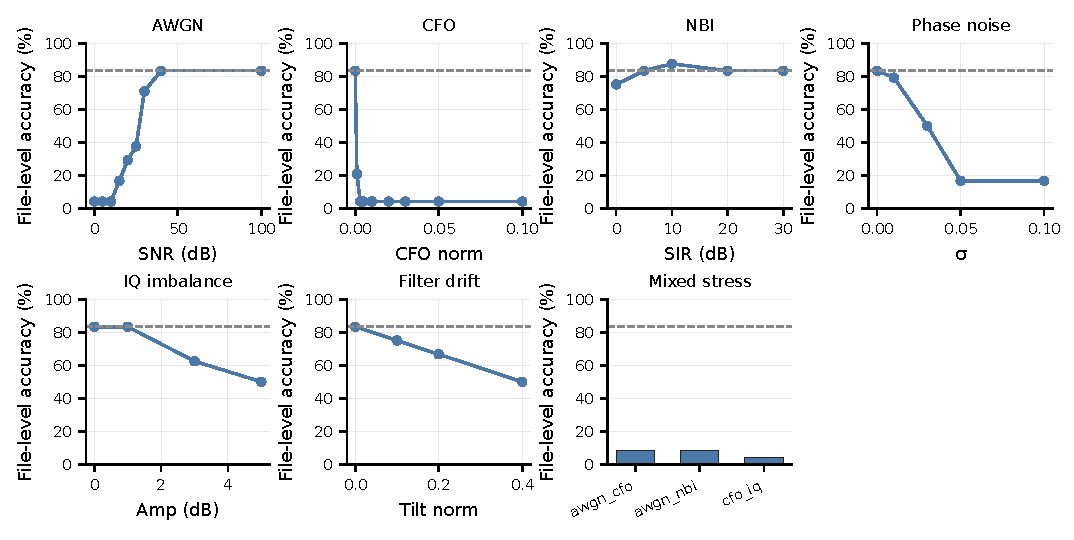
\includegraphics[width=0.9\linewidth]{fig5_1_em_robustness_curves.pdf}
  \caption{闭集 EM 鲁棒性退化曲线（Ours）}
  \label{fig:ch5_em}
\end{figure}

\section{闭集电磁鲁棒性}

Clean \textbf{83.3\%}；AWGN 30\,dB 70.8\%；CFO norm $\geq 0.003$ 约 \textbf{4.2\%}；NBI SIR 10\,dB \textbf{87.5\%}（相对温和）。图~\ref{fig:ch5_rank} 为敏感性排序：CFO/强 AWGN 最强。

\begin{figure}[htbp]
  \centering
  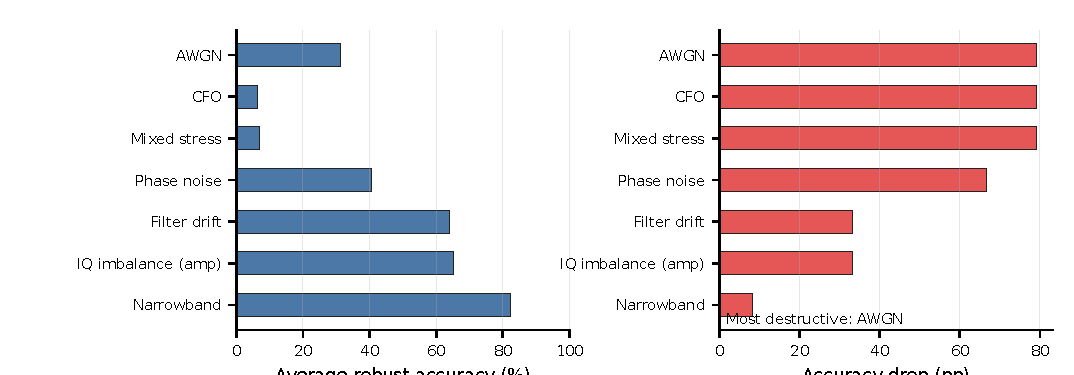
\includegraphics[width=0.75\linewidth]{fig5_3_em_stress_ranking.pdf}
  \caption{扰动敏感性排序}
  \label{fig:ch5_rank}
\end{figure}

\section{CNN-IQ 与 Ours 对比}

表~\ref{tab:ch5_cnn}。Clean 62.5 vs 83.3（+20.8 pp）；NBI 10 dB 29.2 vs 87.5（+58.3 pp）；CFO 0.003 均为 4.2\%——共同失效。

\begin{table}[htbp]
  \centering
  \caption{CNN-IQ 与 Ours 在 EM 下的对比（seed0，\%）}
  \label{tab:ch5_cnn}
  \begin{tabular}{lccc}
    \toprule
    条件 & CNN-IQ & Ours & $\Delta$ (pp) \\
    \midrule
    Clean & 62.5 & 83.3 & +20.8 \\
    AWGN 30\,dB & 62.5 & 70.8 & +8.3 \\
    CFO 0.003 & 4.2 & 4.2 & 0 \\
    NBI 10\,dB & 29.2 & 87.5 & +58.3 \\
    \bottomrule
  \end{tabular}
\end{table}


\begin{figure}[htbp]
  \centering
  \begin{subfigure}{0.32\linewidth}
    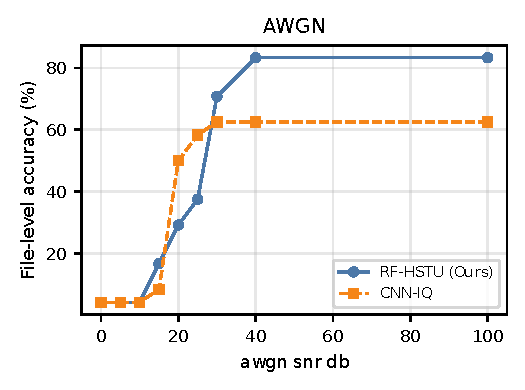
\includegraphics[width=\linewidth]{fig5_cnn_vs_ours_awgn.pdf}
    \caption{AWGN}
  \end{subfigure}
  \begin{subfigure}{0.32\linewidth}
    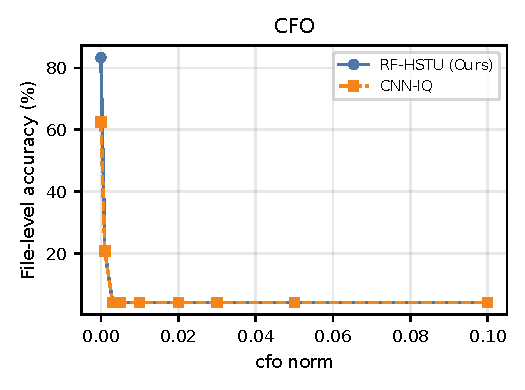
\includegraphics[width=\linewidth]{fig5_cnn_vs_ours_cfo.pdf}
    \caption{CFO}
  \end{subfigure}
  \begin{subfigure}{0.32\linewidth}
    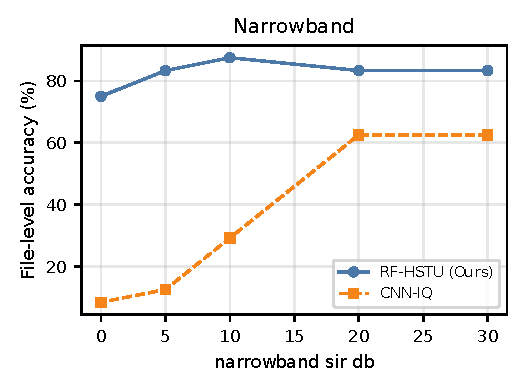
\includegraphics[width=\linewidth]{fig5_cnn_vs_ours_narrowband.pdf}
    \caption{NBI}
  \end{subfigure}
  \caption{CNN-IQ 与 Ours 在 EM 下的对比}
  \label{fig:ch5_cnn}
\end{figure}

\section{开放集未知设备认证}

Prototype AUROC \textbf{$0.917\pm0.059$}，Mahalanobis $0.913\pm0.062$；MSP $0.425$，Energy $0.575$。图~\ref{fig:ch5_os_clean}。

\begin{figure}[htbp]
  \centering
  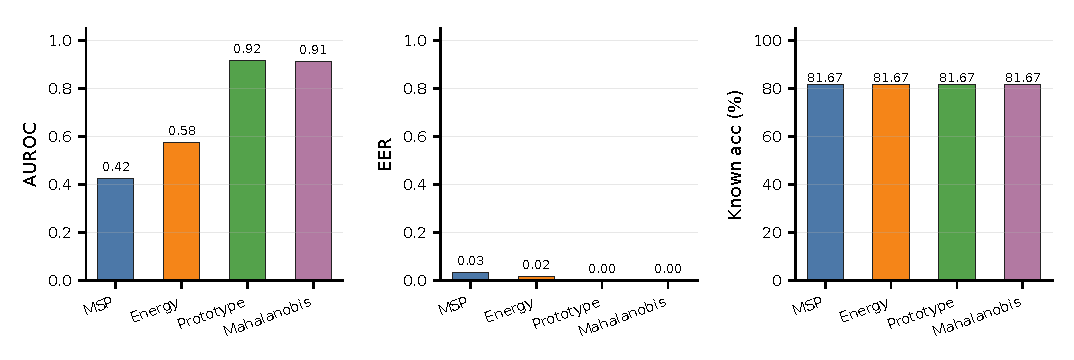
\includegraphics[width=0.8\linewidth]{fig5_2_openset_clean.pdf}
  \caption{Clean open-set 各 scorer 对比}
  \label{fig:ch5_os_clean}
\end{figure}

\section{EM stress 下的 open-set}

图~\ref{fig:ch5_os_em}：AWGN 30 dB Proto AUROC 0.896；CFO 0.003 AUROC \textbf{0.492}，known acc \textbf{3.3\%}——同时摧毁分类与拒识。

\begin{figure}[htbp]
  \centering
  \begin{subfigure}{0.48\linewidth}
    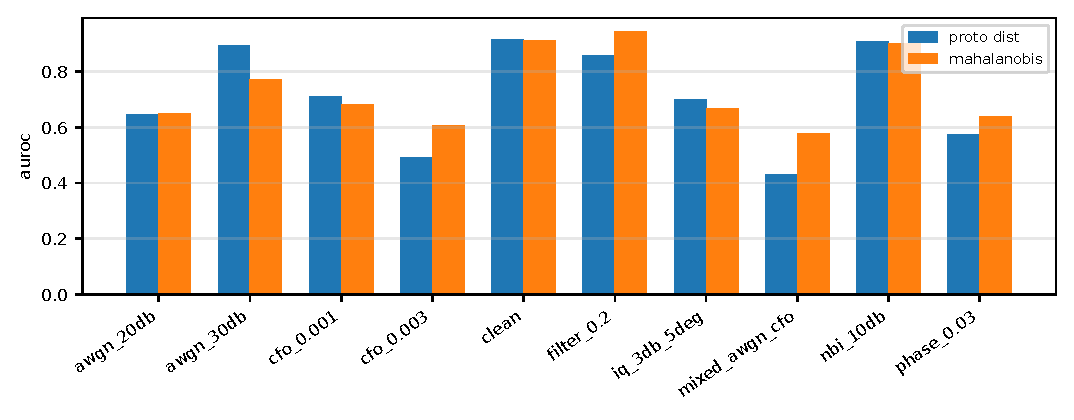
\includegraphics[width=\linewidth]{fig5_4_auroc_under_em.pdf}
    \caption{AUROC under EM}
  \end{subfigure}
  \begin{subfigure}{0.48\linewidth}
    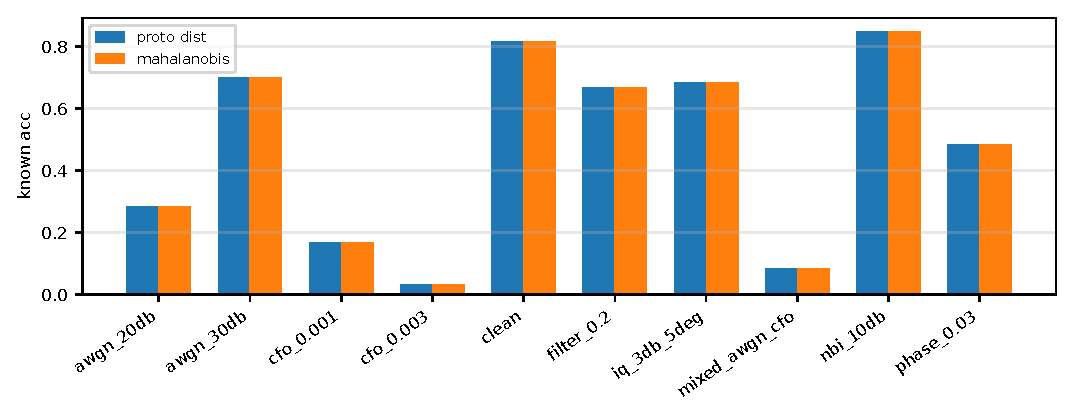
\includegraphics[width=\linewidth]{fig5_6_known_acc_under_em.pdf}
    \caption{Known acc under EM}
  \end{subfigure}
  \caption{开放集在 EM 应力下的退化}
  \label{fig:ch5_os_em}
\end{figure}

\section{EM-CR 初步分析（非主方法）}

扰动一致性微调（EM-CR）为初步探索。强 CFO + 全主干训练致 clean 83.3\%$\rightarrow$20.8\% 崩溃；保守设置（冻结主干、弱扰动）无稳定鲁棒增益。\textbf{不作为第三创新点核心}；后续宜采用课程式增强、teacher-student 等。

表~\ref{tab:ch5_emcr} 为 debug suite 摘要。

\begin{table}[htbp]
  \centering
  \caption{EM-CR debug suite（非主方法，head-only 3 epoch）}
  \label{tab:ch5_emcr}
  \begin{tabular}{lcc}
    \toprule
    变体 & Clean (\%) & AWGN 30\,dB (\%) \\
    \midrule
    A clean-only FT & $\sim$79.2 & -- \\
    B EM-Aug CE & $\sim$79.2 & $\sim$62.5 \\
    C weak CFO aug & -- & 70.8 \\
    D stopgrad KL & $\sim$79.2 & $\sim$62.5 \\
    Smoke（强 CFO+全主干） & \multicolumn{2}{c}{clean 83.3$\rightarrow$20.8（崩溃）} \\
    \bottomrule
  \end{tabular}
\end{table}


\section{本章小结}

本章构建 EM benchmark 与 open-set 协议；CFO 为最强 failure mode；Prototype/Mahalanobis 优于 MSP/Energy；EM-CR 未达主方法标准。

\chapter{总结与展望}
\label{ch:conclusion}

\section{全文工作总结}

本文围绕 LoRa 设备射频指纹在复杂部署条件下的认证可靠性，从跨日建模、跨接收机校准与复杂电磁/open-set 评估三条主线展开，强调可复现协议与诚实失效分析。

\section{创新点回顾}

\textbf{创新点一}：OOB-guided RF-HSTU，cross-day $75.0\pm5.3\%$ vs CNN $54.2\pm14.2\%$。

\textbf{创新点二}：OOB 纠缠诊断 + RCPA-T，$K{=}20$ 时 $75.0\%$ vs source-only $\sim$20\%。

\textbf{创新点三}：EM benchmark + open-set；Proto AUROC $0.917$；CFO 双崩溃；EM-CR 为 future work。

\section{不足与展望}

数据集规模与接收机数量有限；open-set unknown 为 hold-out 设备；CFO 鲁棒性不足；EM-CR 未形成稳定方法。展望：多接收机采集、波形级 CFO 补偿、receiver-statistics 校准、开放集阈值自适应及与 LoRaWAN 认证融合。

\section{本章小结}

本文提供了 LoRa RFFI 从建模到评估的完整链条与性能边界，为后续物理层安全研究提供基准与经验参考。


\backmatter
\bibliographystyle{plain}
\bibliography{refs}

\end{document}
